\centering
	\uncover<2->{
		Maximum number of nodes in memory:
			\alt<2>{0}{\alt<3>{1}{\alt<4>{2}{\alt<5-11>{3}{\alt<12>{0}{\alt<13>{1}{\alt<14>{2}{\alt<15>{3}{\alt<16>{4}{5}}}}}}}}} \\[1cm]
	}
	\begin{minipage}{.5\linewidth}
		\uncover<2->{
		\begin{tikzpicture}[node distance=1.2cm]
			\proofnodeBW{unp};
			\proofnodeBW[below=of unp]{pebbled};
			\whitenode{unp};
			\blacknode{pebbled};
			\node[right =of unp, xshift=-1em] (t1) {Not in memory};
			\node[right =of pebbled, xshift=-1em] (t1) {In memory};
		\end{tikzpicture}
		}
	\end{minipage}%
	\begin{minipage}{.5\linewidth}
	\only<1>{
		\begin{tikzpicture}[node distance=1.2cm]
			\rootnode;
			\withchildren{root}{x1}{$x_1$} {nx1}{$\neg x_1$};
			\withchildren{x1}{n3}{$x_1,x_3$} {n4} {$x_1, \neg x_3$};
			\withchildren{n3}{n1}{$x_1,x_2, x_3$} {n4} {$x_1, \neg x_2$};
		\end{tikzpicture}
	}
	\only<2->{
		\begin{tikzpicture}[node distance=1.2cm]
				\rootnodeBW;
				\withchildrenBW{root} {n5}  {n6};
				\addchildrenBW{n5}   {n3} {n4};
				\drawchildren{n5} {n3} {n4};
				\withchildrenBW{n3} {n1} {n2};
				\blacknode<3,4,5,15,16,17>{n1};
				\blacknode<4,5,16,17>{n2};
				\blacknode<5,6,7,8,17,18,19>{n3};
				\blacknode<7,8,14-19>{n4};
				\blacknode<8,9,10,11,19->{n5};
				\blacknode<10,11,13->{n6};
				\blacknode<11,21->{root};
		\end{tikzpicture}
		}
	\end{minipage}%
